% Classes of src/core/Math/Fitting and their dependencies. Paper: section "Fitting" (fig:fitting); Doxygen: Fitter.hpp.
%   pdflatex FittingClasses.tex; pdftoppm -r 200 -png -singlefile FittingClasses.pdf FittingClasses;
%   pdftocairo -svg FittingClasses.pdf FittingClasses.svg
\documentclass[tikz,border=2pt]{standalone}
% Shared style of the class diagrams of CAP (figures/*Classes.tex): \input after \documentclass[tikz]{standalone}.
%  - boxes: blue = abstract base class, light blue = class, green = entry class of the folder (steering class, task),
%    yellow = free functions (tools), grey = class of another folder;
%  - arrows: open triangle = inherits from; dashed with diamond = owns (holds); dashed with arrow = uses.
\usepackage[scaled=0.92]{helvet}
\usetikzlibrary{arrows.meta,shapes.multipart,positioning,fit,backgrounds,calc}
\renewcommand{\familydefault}{\sfdefault}
\definecolor{abstract}{HTML}{D6E4F5}
\definecolor{concrete}{HTML}{EEF4FB}
\definecolor{steer}{HTML}{DCEFD9}
\definecolor{tools}{HTML}{FFF8E6}
\definecolor{external}{HTML}{E9E9E9}
\definecolor{dependline}{HTML}{8A6D3B}
\definecolor{folder}{HTML}{F7F7F7}
\tikzset{
  every picture/.style={font=\scriptsize},
  cls/.style={draw, fill=concrete, align=center, inner sep=2.5pt, text width=#1, font=\tiny},
  cls/.default=3.0cm,
  abs/.style={cls=#1, fill=abstract},
  abs/.default=3.0cm,
  steer/.style={cls=#1, fill=steer, line width=0.8pt},
  steer/.default=4.2cm,
  tool/.style={cls=#1, fill=tools},
  tool/.default=4.2cm,
  ext/.style={cls=#1, fill=external, dashed},
  ext/.default=2.6cm,
  fam/.style={draw, rectangle split, rectangle split parts=2, rectangle split part fill={#1,white},
              rectangle split part align={center,left}, inner sep=2.5pt, align=left},
  inherit/.style={-{Triangle[open,length=2.2mm,width=2.2mm]}, thin},
  uses/.style={dashed, dependline, -{Stealth[length=1.6mm]}, thin},
  owns/.style={dashed, dependline, {Diamond[length=2.4mm,width=1.6mm]}-, thin},
  lbl/.style={font=\tiny, text=dependline, align=center},
  note/.style={font=\tiny, align=left, text=black!70},
  title/.style={font=\footnotesize\bfseries, anchor=north west},
}
% a member line in a class box
\newcommand{\m}[1]{\\#1}
\newcommand{\cn}[1]{{\scriptsize\textbf{#1}}}
\newcommand{\an}[1]{{\scriptsize\textbf{\textit{#1}}}}

% legend common to the class diagrams (place with \legendat{x}{y})
\newcommand{\legendat}[2]{%
  \begin{scope}[shift={(#1,#2)}, font=\tiny]
    \node[abs=0.9cm, minimum height=3mm, inner sep=1pt] (lA) at (0,0) {abstract};
    \node[cls=0.9cm, minimum height=3mm, inner sep=1pt, right=1mm of lA] (lC) {class};
    \node[steer=1.1cm, minimum height=3mm, inner sep=1pt, right=1mm of lC] (lS) {entry class};
    \node[tool=1.1cm, minimum height=3mm, inner sep=1pt, right=1mm of lS] (lT) {functions};
    \node[ext=1.3cm, minimum height=3mm, inner sep=1pt, right=1mm of lT] (lE) {other folder};
    \draw[inherit] ($(lE.east)+(1mm,0)$) -- ++(5mm,0) node[right, inner sep=1pt] (l1) {inherits};
    \draw[owns] ($(l1.east)+(1mm,0)$) -- ++(5mm,0) node[right, inner sep=1pt] (l2) {owns};
    \draw[uses] ($(l2.east)+(1mm,0)$) -- ++(5mm,0) node[right, inner sep=1pt] {uses};
  \end{scope}}

\begin{document}
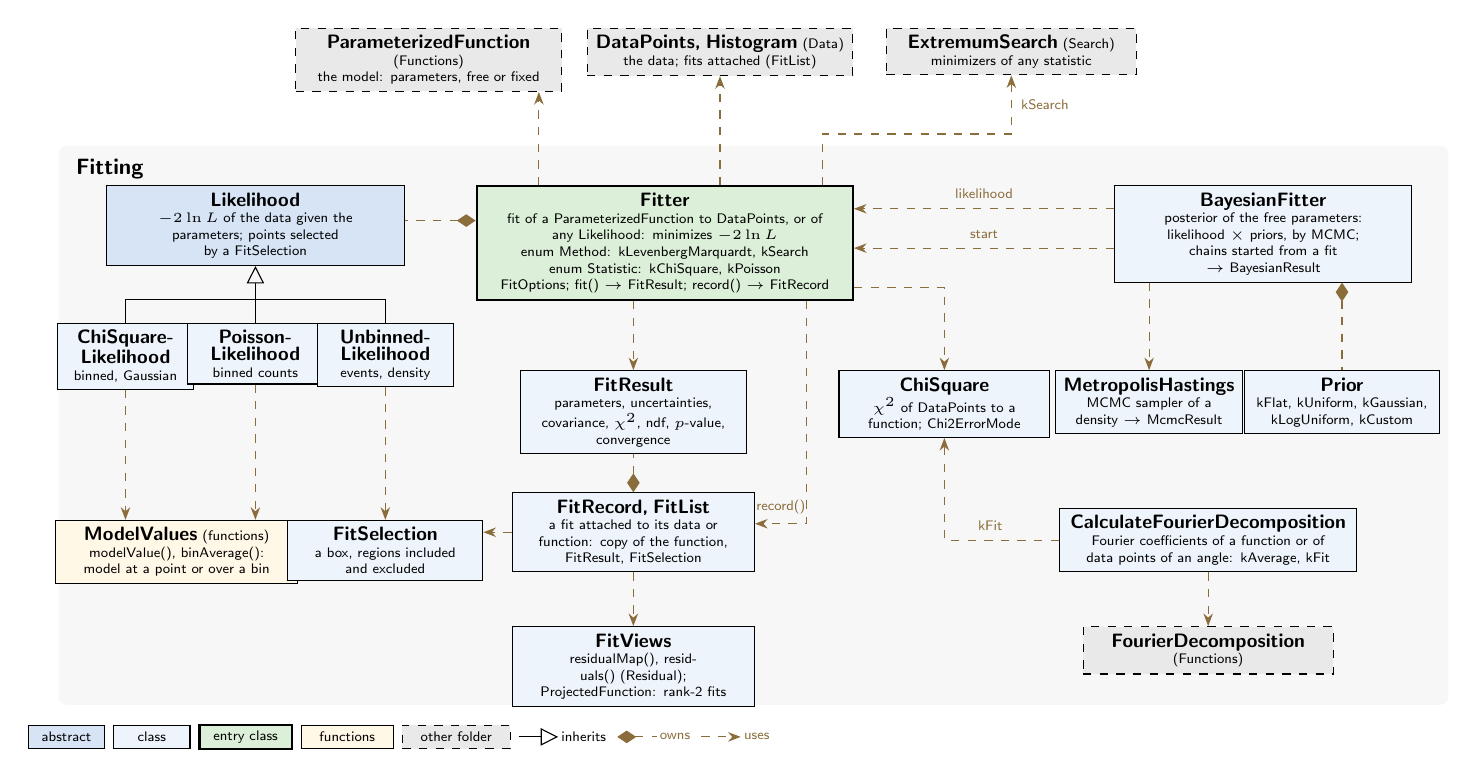
\begin{tikzpicture}[every node/.append style={anchor=north}]
  \begin{scope}[on background layer]
    \fill[folder, rounded corners=3pt] (-0.1,-1.15) rectangle (17.55,-8.25);
  \end{scope}
  \node[title] at (0.0,-1.2) {Fitting};

  % other folders, top
  \node[ext=3.2cm] (PF) at (4.6,0.35) {\an{ParameterizedFunction} \tiny(Functions)\m{the model: parameters, free or fixed}};
  \node[ext=3.2cm] (DP) at (8.3,0.35) {\cn{DataPoints, Histogram} \tiny(Data)\m{the data; fits attached (FitList)}};
  \node[ext=3.0cm] (ES) at (12.0,0.35) {\cn{ExtremumSearch} \tiny(Search)\m{minimizers of any statistic}};

  % fitting
  \node[steer=4.6cm] (Fitter) at (7.6,-1.65)
    {\cn{Fitter}\m{fit of a ParameterizedFunction to DataPoints, or of}\m{any Likelihood: minimizes $-2\ln L$}
     \m{enum Method: kLevenbergMarquardt, kSearch}\m{enum Statistic: kChiSquare, kPoisson}
     \m{FitOptions; fit() $\to$ FitResult; record() $\to$ FitRecord}};
  \node[abs=3.6cm] (Lik) at (2.4,-1.65)
    {\an{Likelihood}\m{$-2\ln L$ of the data given the}\m{parameters; points selected}\m{by a FitSelection}};
  \node[cls=1.55cm] (CSL) at (0.75,-3.4) {\cn{ChiSquare-}\\\cn{Likelihood}\m{binned, Gaussian}};
  \node[cls=1.55cm] (PL) at (2.4,-3.4) {\cn{Poisson-}\\\cn{Likelihood}\m{binned counts}};
  \node[cls=1.55cm] (UL) at (4.05,-3.4) {\cn{Unbinned-}\\\cn{Likelihood}\m{events, density}};
  \draw (CSL.north) |- (2.4,-3.1) (UL.north) |- (2.4,-3.1);
  \draw[inherit] (PL.north) -- (Lik.south);
  \node[tool=2.9cm] (MV) at (1.4,-5.9) {\cn{ModelValues} \tiny(functions)\m{modelValue(), binAverage():}\m{model at a point or over a bin}};
  \node[cls=2.3cm] (Sel) at (4.05,-5.9) {\cn{FitSelection}\m{a box, regions included}\m{and excluded}};
  \draw[uses] (CSL.south) -- (CSL.south |- MV.north);
  \draw[uses] (PL.south) -- (PL.south |- MV.north);
  \draw[uses] (UL.south) -- (UL.south |- Sel.north);

  \node[cls=2.7cm] (FR) at (7.2,-4.0) {\cn{FitResult}\m{parameters, uncertainties,}\m{covariance, $\chi^2$, ndf, $p$-value,}\m{convergence}};
  \node[cls=2.9cm] (Rec) at (7.2,-5.55) {\cn{FitRecord, FitList}\m{a fit attached to its data or}\m{function: copy of the function,}\m{FitResult, FitSelection}};
  \node[cls=2.9cm] (Views) at (7.2,-7.25) {\cn{FitViews}\m{residualMap(), residuals() (Residual);}\m{ProjectedFunction: rank-2 fits}};
  \node[cls=2.5cm] (Chi) at (11.15,-4.0) {\cn{ChiSquare}\m{$\chi^2$ of DataPoints to a}\m{function; Chi2ErrorMode}};

  \draw[owns] (Fitter.west |- 0,-2.1) -- (Lik.east |- 0,-2.1);
  \draw[uses] (7.2,0 |- Fitter.south) -- (FR.north);
  \draw[uses] (9.4,0 |- Fitter.south) -- (9.4,-5.95) -- node[lbl, above]{record()} (Rec.east |- 0,-5.95);
  \draw[owns] (Rec.north) -- (FR.south);
  \draw[uses] (Rec.south) -- (Views.north);
  \draw[uses] (Rec.west) -- (Rec.west -| Sel.east);
  \draw[uses] (6.0,0 |- Fitter.north) -- (6.0,0 |- PF.south);
  \draw[uses] (8.3,0 |- Fitter.north) -- (DP.south);
  \draw[uses] (9.6,0 |- Fitter.north) -- (9.6,-1.0) -| node[lbl, pos=0.75, right]{kSearch} (ES.south);
  \draw[uses] (Fitter.east |- 0,-2.95) -| (Chi.north);

  % Bayesian
  \node[cls=3.6cm] (Bayes) at (15.2,-1.65)
    {\cn{BayesianFitter}\m{posterior of the free parameters:}\m{likelihood $\times$ priors, by MCMC;}
     \m{chains started from a fit}\m{$\to$ BayesianResult}};
  \node[cls=2.3cm] (Prior) at (16.2,-4.0) {\cn{Prior}\m{kFlat, kUniform, kGaussian,}\m{kLogUniform, kCustom}};
  \node[cls=2.2cm] (MH) at (13.75,-4.0) {\cn{MetropolisHastings}\m{MCMC sampler of a}\m{density $\to$ McmcResult}};
  \draw[owns] (16.2,0 |- Bayes.south) -- (Prior.north);
  \draw[uses] (13.75,0 |- Bayes.south) -- (MH.north);
  \draw[uses] (Bayes.west |- 0,-2.45) -- node[lbl, above]{start} (Fitter.east |- 0,-2.45);
  \draw[uses] (Bayes.west |- 0,-1.95) -- node[lbl, above]{likelihood} (Fitter.east |- 0,-1.95);

  \node[cls=3.6cm] (CFD) at (14.5,-5.75)
    {\cn{CalculateFourierDecomposition}\m{Fourier coefficients of a function or of}\m{data points of an angle: kAverage, kFit}};
  \node[ext=3.0cm] (FD) at (14.5,-7.25) {\cn{FourierDecomposition}\m{(Functions)}};
  \draw[uses] (CFD.south) -- (FD.north);
  \draw[uses] (CFD.west) -| node[lbl, pos=0.3, above]{kFit} (Chi.south);
  \legendat{0.0}{-8.5}
\end{tikzpicture}
\end{document}
